\chapter{Resultados}

Este capítulo tem como objetivo apresentar as estratégias usadas para projetar e refinar o controle PID empregado no ajuste automático da luminosidade no modo ``Econômico'', mostrar o comportamento do controlador diante de algumas métricas comumente usadas para avaliar sistema de controle como sua resposta ao degrau e integral do erro, e apresentar valores estimados de consumo de energia em cenários de uso com os modos ``Normal'' e ``Econômico''. 
% Talvez não seja necessário falar isso daqui pra baixo
A demonstração das outras funcionalidades do sistema (ligar e desligar via internet, por exemplo) são triviais para que sejam mostradas de forma escrita.

\section{Sintonia e Ajustes do controle de luminosidade}

Para sintonizar as constantes do controlador PID foi utilizada a técnica de Ziegler-Nichols. Dado um porto de partida da sintonia, alguns ajustes foram feitos de forma empírica visando minimizar o \textit{overshoot}, o tempo de subida e as oscilações em regime permanente.

O método de Ziegler-Nichols é um método empírico de caracterização da planta e determinação dos parâmetros do controlador PID. O método consiste, como descrito anteriormente, na obtenção de dois parâmetros da planta: O ganho crítico, denotado por $K_{cr}$, e o período de oscilação crítico, $T_{cr}$. Os parâmetros obtidos foram:
\begin{equation}
    \label{eq:rs1}
    K_{cr} = 1.6
\end{equation}
\begin{equation}
    \label{eq:rs1.1}
    T_{cr} = 3 s.
\end{equation}

O desempenho do controlador foi avaliado para as três sintonias mais comuns oriundas do método de Ziegler-Nichols de acordo  com a Tabela \ref{ZN}.

\begin{table}[htb]
    \centering
    \caption{Resultados de sintonia de Ziegler-Nichols}
    \label{ZNvalores}
    \begin{tabular}{llll}
    \hline
    Tipo            & $K_P$ & $K_I$ & $K_D$ \\ 
    \hline \hline
    Clássico        & $0,72$ & $0,64$ & $0.36$ \\ 
    \hline
    Overshoot baixo & $0,53$ & $0,64$ & $0,96$ \\ 
    \hline
    Sem overshoot   & $0,32$ & $0,64$ & $0,96$ \\
    \hline
    \end{tabular}
\end{table}

Os comportamentos obtidos de resposta ao degrau do controlador com as sintonias listadas na Tabela \ref{ZNvalores} podem ser observados nas Figuras \ref{znclass}, \ref{znpo} e \ref{znso} respectivamente.
\begin{figure}[ht]
    \begin{center}
    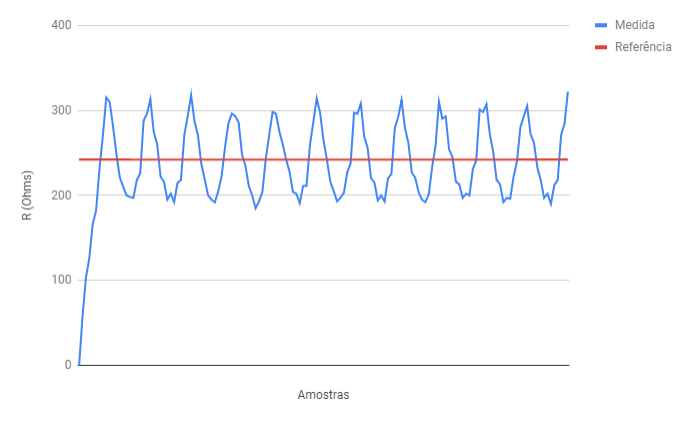
\includegraphics[width=0.75\textwidth]{figuras/znclass.PNG}
    \end{center}
    \caption[Gráfico da sintonia clássica de Ziegler-Nichols.]{Gráfico da resposta ao degrau da sintonia clássica de Ziegler-Nichols com alta oscilação em regime permanente.}
    \label{znclass}
\end{figure}
\begin{figure}[ht]
    \begin{center}
    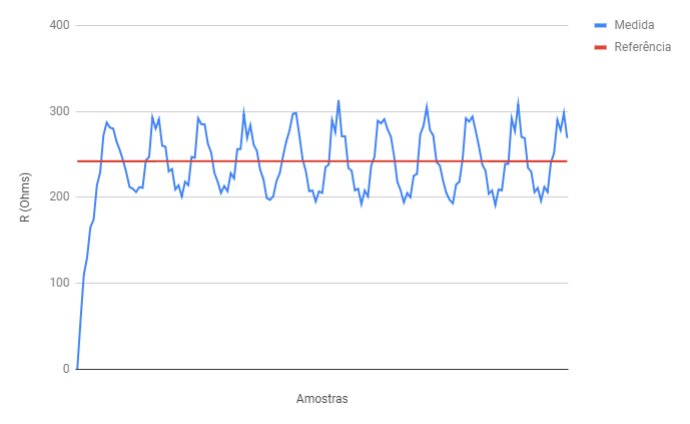
\includegraphics[width=0.75\textwidth]{figuras/znpo.PNG}
    \end{center}
    \caption[Gráfico da sintonia de Ziegler-Nichols ``com pouco overshoot''.]{Gráfico da resposta ao degrau da sintonia de Ziegler-Nichols ``com pouco overshoot'', ainda assim com alta oscilação em regime permanente.}
    \label{znpo}
\end{figure}
\begin{figure}[ht]
    \begin{center}
    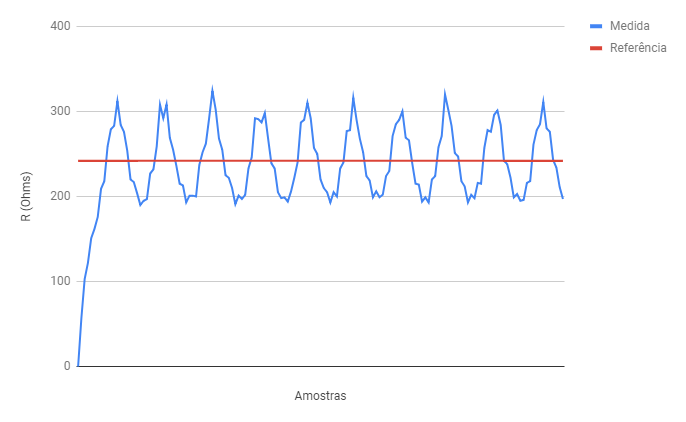
\includegraphics[width=0.75\textwidth]{figuras/znso.PNG}
    \end{center}
    \caption[Gráfico da sintonia de Ziegler-Nichols ``sem overshoot''.]{Gráfico da resposta ao degrau da sintonia de Ziegler-Nichols ``sem overshoot'', ainda assim com alta oscilação em regime permanente.}
    \label{znso}
\end{figure}

Pode-se notar que as sintonias citadas aplicadas ao controlador PID apresentam comportamento instável já que a oscilação em regime permanente não converge a zero. Tendo em vista o forte comportamento oscilatório, os ganhos integral e derivativo foram diminuídos ao ponto que o comportamento oscilatório não era mais observado, dando ao controlador um comportamento sub-amortecido, e em seguida o ganho proporcional foi incrementado até observar o aparecimento de \textit{overshoot}. A sintonia obtida nesta situação pode ser observada na Figura \ref{znsint}. 
\begin{align}
  &K_P = 1 \nonumber\\
  &K_I = 0,08 \nonumber\\
  &K_D = 0,16. \nonumber
\end{align}

\begin{figure}[ht]
    \begin{center}
    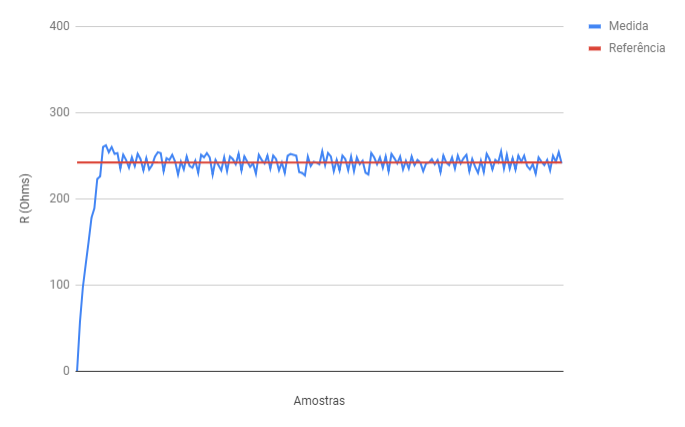
\includegraphics[width=0.75\textwidth]{figuras/znsint.PNG}
    \end{center}
    \caption[Gráfico do controlador PID satisfatoriamente sintonizado.]{Gráfico da resposta ao degrau do controlador PID satisfatoriamente sintonizado.}
    \label{znsint}
\end{figure}

O método de sintonia de Ziegler-Nichols provou ser útil como um ponto de partida da sintonia do controlador pois o resultado apresentado pelo método não foi satisfatório pois apresentava comportamento instável. A partir do resultado obtido pelo método foram feitos ajustes de modo a trazer o controlador para um comportamento estável e com características desejadas (baixo tempo de estabilização e pequeno \textit{overshoot}).

\subsection{Desempenho do controlador PID}

A fim de demonstrar o comportamento do controlador para diversos níveis de luminosidade, diversos níveis de referência foram aplicados ao sistema de forma sequencial começando por um valor maior de luminosidade e diminui por passos discretos até um quarto valor de luminosidade como pode ser observado na Figura \ref{pidstep}. Os valores de luminosidade são representados pela resistência medida do sensor LDR, cuja medida é inversamente proporcional ao valor da luminosidade.

\begin{figure}[ht]
    \begin{center}
    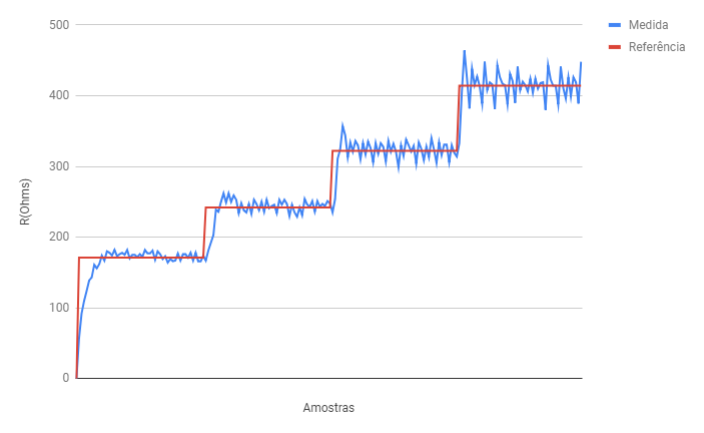
\includegraphics[width=0.75\textwidth]{figuras/pidstep.PNG}
    \end{center}
    \caption[Gráfico do teste de desempenho do controlador PID.]{Gráfico do teste de desempenho do controlador PID com quatro valores discretos de referência.}
    \label{pidstep}
\end{figure}

É importante notar que o desempenho do controlador varia com a região de controle, o que evidencia a não-linearidade já exposta do sistema em função da relação logarítmica da luminosidade medida e da resistência apresentada pelo sensor. Essa relação é apresentada no gráfico disponibilizado na folha de dados do sensor da Figura \ref{reta}, mas a própria folha de dados \cite{ldr} explica que tal comportamento pode variar por diversos fatores como temperatura, fabricação e outros tantos. Portanto é inviável adicionar esse comportamento no modelo de controle. Algumas estratégias de controle como controle adaptativo, controle \textit{fuzzy} e outras abordagens modernas conseguem lidar com esse tipo de não-linearidade, mas no caso desse trabalho decidiu-se adotar uma abordagem clássica PID de forma que o controle fosse ainda estável no pior caso, ainda que não apresentasse uma performance satisfatória.  

\section{Economia de Energia}

O fato de o sistema de iluminação apresentado poder ter sua intensidade luminosa regulada numa escala de zero a cem por cento da luminosidade máxima da fonte luminosa representa, além de outras vantagens, uma capacidade de economia de energia. A percepção humana de luminosidade, assim como a audição, tem um caráter logarítmico e isto significa que variações de luminosidade em um patamar de alta intensidade são percebidas de forma mais pobre do que as mesmas variações em patamares de baixa luminosidade. Muitas vezes, a luminosidade máxima de uma fonte provocaria sensação de intensidade semelhante a 80$\%$ ou 70$\%$ da luminosidade máxima e a possibilidade de regular a intensidade para tais valores menores que o máximo mas ainda confortáveis, pode economizar energia sem comprometer o conforto.

Buscando exemplificar a capacidade de economia de energia de sistema foram analisados dois dias distintos de uso do sistema com o modo econômico em sua maior parte. Os gráficos nas Figuras \ref{gren1} e \ref{gren2} representam, respectivamente, as porcentagens da intensidade máxima do sistema de iluminação momentâneas amostradas a cada trinta segundos durante 24 horas. O primeiro gráfico é do uso durante o dia 23 de outubro e o segundo gráfico é do uso durante o dia 29 de outubro.
\begin{figure}[htb]
    \begin{center}
    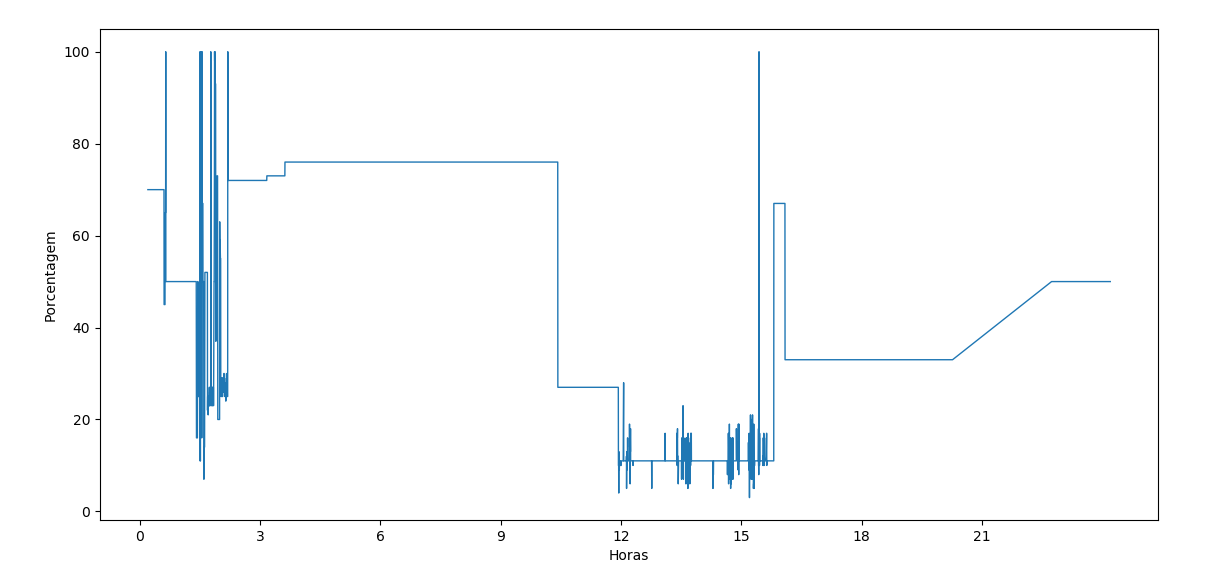
\includegraphics[width=0.85\textwidth]{figuras/gren1.PNG}
    \end{center}
    \caption[Gráfico do consumo relativo durante o dia 23 de outubro.]{Gráfico do consumo relativo durante o dia 23 de outubro.}
    \label{gren1}
\end{figure}
\begin{figure}[htb]
    \begin{center}
    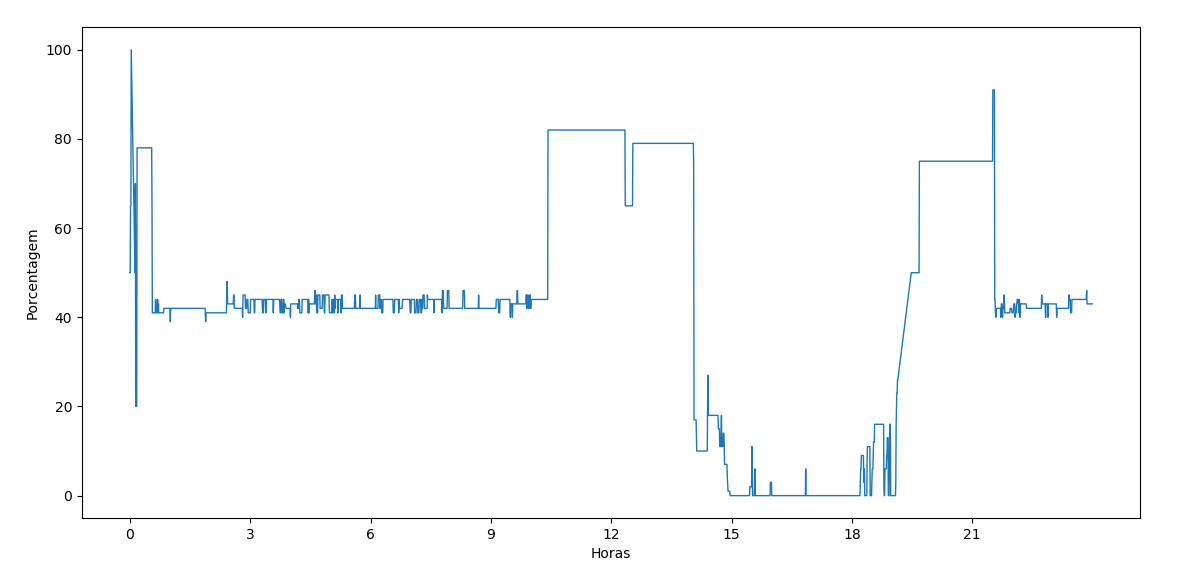
\includegraphics[width=0.85\textwidth]{figuras/gren2.PNG}
    \end{center}
    \caption[Gráfico do consumo relativo durante o dia 29 de outubro.]{Gráfico do consumo relativo durante o dia 29 de outubro.}
    \label{gren2}
\end{figure}

O sistema permaneceu ligado durante as 24 horas observadas nas duas situações, a potência assumiu valores nulos apenas em momentos em que a luminosidade do ambiente, independente da contribuição da fita de LED, superava o valor de referência e o controlador atingia uma condição de saturação. 

O consumo de energia pode ser representado como um valor relativo ao consumo hipotético da mesma fonte luminosa com capacidade máxima, ou 100\% da intensidade máxima. O cálculo da energia consumida é feito a partir da integração numérica da potência relativa instantânea de acordo com a equação \eqref{eq:en_6}. O valor relativo de energia consumida na primeira situação foi de 46.5\% e na segunda foi de 43.3\%. 
